%
% Copyright (c) 2011-2013, fortiss GmbH.
% Licensed under the Apache License, Version 2.0.
% 
% Use, modification and distribution are subject to the terms specified
% in the accompanying license file LICENSE.txt located at the root directory
% of this software distribution. A copy is available at
% http://chromosome.fortiss.org/.
%
% This file is part of CHROMOSOME.
%
% $Id: example_helloworld.tex 5238 2013-09-30 15:44:39Z ruiz $
%

\section{Example 5: Calculator Server (15 minutes)}
\label{sec:example_calculator}

The next example demonstrates the use of an alternative communication pattern provided by \xme,
the so-called request/response (or RR) style of communication.
In contrast to publish/subscribe, which has basically a fire \& forget semantics,
RR works more like client/server:
components can send \emph{requests} that can be processed by one or more \emph{request handlers}.
On success, the request handler sends a \emph{response} back to the component that issued the request.

For this purpose, two topics are required: a request topic and a response topic.
A data packet of type request is sent from the client to the server ``on demand''
and contains all information necessary for the server to process the request.
Subsequently, the server shall reply with a data packet of type response, which contains the server's answer.

Unlike in ``normal'' publish/subscribe, where all subscribers would receive all kind of data that match their topic,
the response is only sent to the component that sent the respective request.
Hence, this communication pattern is useful to query a component for a value at an irregular frequency or even once only.

\subsection{Inspecting the calculator model}

In order to demonstrate the request/response communication pattern,
this release of \xme ships with a second example, which is called \emph{calculator}.

The scenario in this example is ``calculator service'' that allows to answer simple calculation queries.
The request topic consists of two operands and one of the operations addition, subtraction, multiplication and division.
When a request is sent to a calculator server, the server shall reply with the result of the requested operation.

The example contains a calculator server node and two ``clients'' that send random requests at regular intervals.
Both clients and servers display their current status (sent requests, processed requests, and received responses) on their standard output.

In order to inspect the example, import the \emph{calculator} project into XMT as you have previously done it with the \emph{sensorMonitor} example
(see Section~\ref{sec:example_xmt}).
From the \emph{models} folder, open the file \emph{deployment.xmn}.

Let's first have a look at the topics that are defined in this example by clicking on the \emph{Topics} tab of the loaded deployment
(compare Figure~\ref{fig:xmt_calculator_topics}).
As you can see, there is a \emph{calculatorRequest} topic and a \emph{calculatorResponse} topic defined.

The \emph{calculatorRequest} topic contains two operands of type \emph{int32\_t} as well as an enumeration called \emph{operation},
which can be one of the four basic arithmetic operations.
%
The \emph{calculatorResponse} topic just contains a double-precision floating-point value named \emph{result}.

\begin{figure}[htpb]
	\centering
	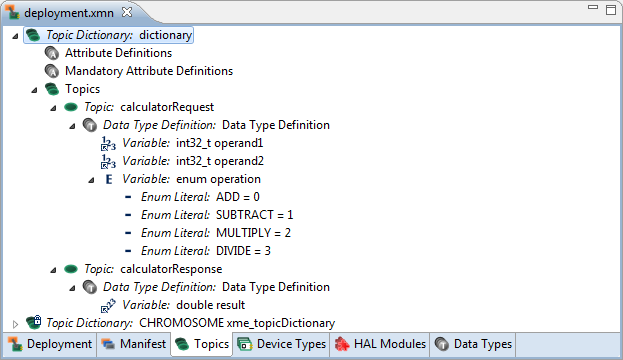
\includegraphics[scale=0.75]{figures/xmt_calculator_topics.png}
	\caption{Topic model of the \emph{calculator} example.}
	\label{fig:xmt_calculator_topics}
\end{figure}

Next, let's have a look at the component manifest of the \emph{calculator} example (compare Figure~\ref{fig:xmt_calculator_manifest}).
It lists two application-specific components:
\begin{itemize}
	\item A \emph{Calculator} component waits for client requests and handles them as they arrive.
		Furthermore, it provides respective output on the console.
	
	\item A \emph{Client} component sends a request using random numbers and operations and displays both request and response in its console.
\end{itemize}
%
\begin{figure}[htpb]
	\centering
	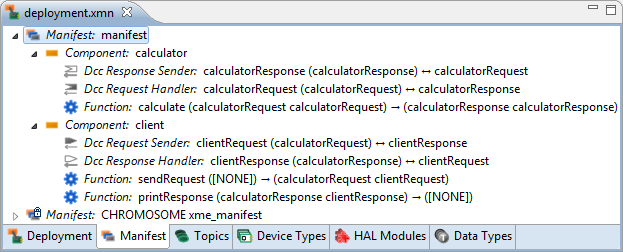
\includegraphics[scale=0.75]{figures/xmt_calculator_manifest.png}
	\caption{Component manifest of the \emph{calculator} example.}
	\label{fig:xmt_calculator_manifest}
\end{figure}
%
Using this simple setup, we can build a deployment model with three nodes as shown on Figure~\ref{fig:xmt_calculator_deployment}.
Notice that we instantiated the \emph{Client} component twice, both on \emph{client1Node} and on \emph{client2Node}.
This means that when we start the applications, requests will be sent to \emph{serverNode} from both client nodes,
but a response will only be delivered to the node that actually sent the request.
%
You might wonder why we need two client nodes. Could not we just launch the same compiled node twice?
Since the address of a node is hard-coded into its executable in this example, we cannot do that.
Otherwise, the server would be unable to distinguish between the two clients
and the used UDP port for communication would be already occupied by the other client process.

\begin{figure}[htpb]
	\centering
	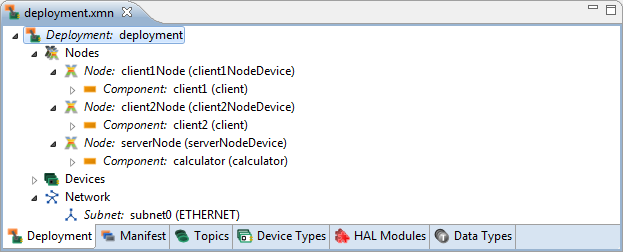
\includegraphics[scale=0.75]{figures/xmt_calculator_deployment.png}
	\caption{Deployment model of the \emph{calculator} example.}
	\label{fig:xmt_calculator_deployment}
\end{figure}

Now it's time to build the node files and run the example.
%
You should be able to build the nodes from within XMT by right-clicking on the root element in the deployment model and selecting \emph{Build Application...}.
In the build window, select the options according to Figure~\ref{fig:xmt_calculator_buildWindow}.
Notice that you need to setup the setting under \emph{Window} $\rightarrow$ \emph{Preferences} $\rightarrow$ \emph{XMT} $\rightarrow$ \emph{CMake}
correctly for this to work (using \emph{Visual Studio 10} as generator is recommended if you have Visual Studio 2010 installed).
Check the output in the XMT console window for any problems such as error messages.

\begin{figure}[htpb]
	\centering
	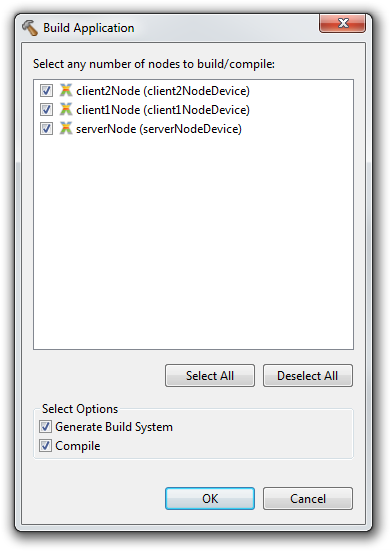
\includegraphics[scale=0.75]{figures/xmt_calculator_buildWindow.png}
	\caption{XMT build options for the \emph{calculator} example.}
	\label{fig:xmt_calculator_buildWindow}
\end{figure}

If this does not work as expected, follow the instructions from Section~\ref{sec:example_sensorMonitor:linux} (Linux)
or~\ref{sec:example_sensorMonitor:windows} (Windows) to manually create the build system and compile each of the three nodes
(\emph{serverNode}, \emph{client1Node} and \emph{client2Node}).

Now you can find the compiled executables in the following folders, where \texttt{<node>} is the name of the respective node:
\texttt{<XME\_ROOT>/examples/calculator/build/<node>/target/}.
%
On Windows, select the subfolder corresponding to the appropriate configuration name (usually \emph{Debug}).
You should find an executable in each of these folders, named like the node itself.
First run the \emph{serverNode} executable in order to start the calculator ``daemon''.
Subsequently, run \emph{client1Node} and \emph{client2Node} (in arbitrary order) to see them interact with the server.
The output should look similar to the one shown in Figures~\ref{fig:example_calculator_serverNode}, \ref{fig:example_calculator_client1Node}
and~\ref{fig:example_calculator_client2Node}.

Feel free to inspect the source code of the nodes, which you will find in the directory \texttt{<XME\_ROOT>/examples/calculator/src}.
The individual functions are implemented in the following files inside that directory:
\texttt{calculator/adv/client/src/sendRequestFunction.c} (\emph{sendRequest} function),
\texttt{calculator/adv/calculator/src/calculateFunction.c} (\emph{calculate} function) and
\texttt{calculator/adv/client/src/printResponseFunction.c} (\emph{printResponse} function).

\begin{figure}[htpb]
	\centering
	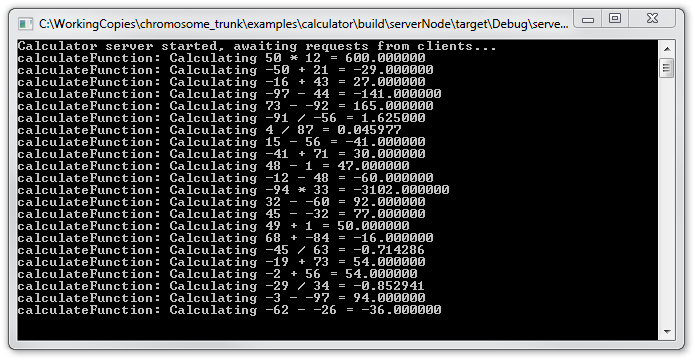
\includegraphics[scale=0.7]{figures/example_calculator_serverNode.png}
	\caption{Console window of \emph{serverNode}.}
	\label{fig:example_calculator_serverNode}
\end{figure}

\begin{figure}[htpb]
	\centering
	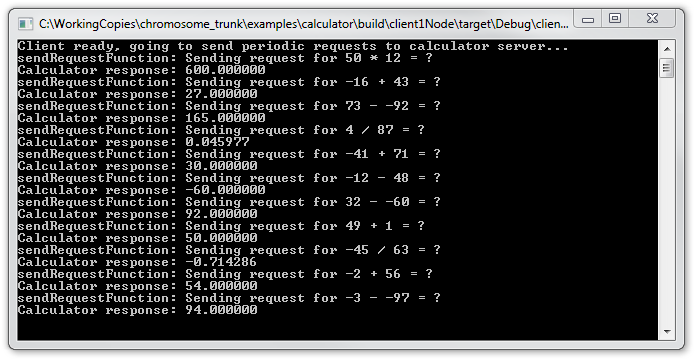
\includegraphics[scale=0.7]{figures/example_calculator_client1Node.png}
	\caption{Console window of \emph{client1Node}.}
	\label{fig:example_calculator_client1Node}
\end{figure}

\begin{figure}[htpb]
	\centering
	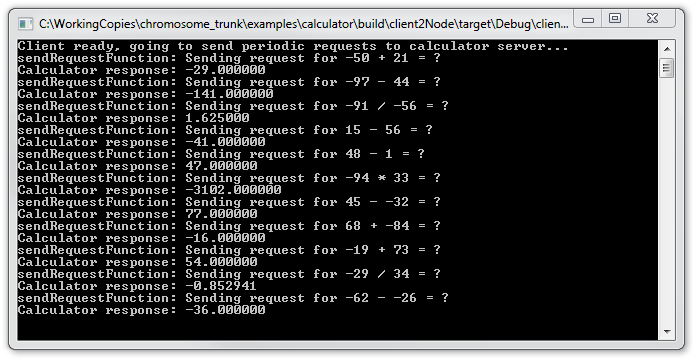
\includegraphics[scale=0.7]{figures/example_calculator_client2Node.png}
	\caption{Console window of \emph{client2Node}.}
	\label{fig:example_calculator_client2Node}
\end{figure}
